\documentclass[11pt,a4paper,openright,twoside]{report}

\usepackage[pdftex]{graphicx}
\usepackage[english]{babel}
\usepackage[T1]{fontenc}
\usepackage[utf8]{inputenc}
\usepackage{url}
\usepackage{setspace}
\usepackage[usenames, dvipsnames]{color}

\usepackage{fancyhdr}
\usepackage{indentfirst}
\usepackage{newlfont}

\usepackage{amssymb}
\usepackage{amsmath}
\usepackage{latexsym}
\usepackage{amsthm}

% for code blocks highlighting
\usepackage{listings}
\usepackage{color}

\definecolor{forestgreenweb}{rgb}{0.13, 0.55, 0.13}
\definecolor{bostonuniversityred}{rgb}{0.8, 0.0, 0.0}
\definecolor{battleshipgrey}{rgb}{0.52, 0.52, 0.51}
\definecolor{whitesmoke}{rgb}{0.96, 0.96, 0.96}

% set the default code style
\lstset{
  language={Python},
  backgroundcolor=\color{whitesmoke},
  basicstyle=\fontsize{7}{7}\ttfamily,
  columns=fullflexible,
  captionpos=b, % Position of the Caption (t for top, b for bottom)
  extendedchars=true, % Allows 256 instead of 128 ASCII characters
  tabsize=4, % number of spaces indented when discovering a tab
  breaklines=true, % wrap lines if they don't fit
  frame=trbl, % draw a frame at the top, right, left and bottom of the listing
  numbers=left, % show line numbers at the left
  morekeywords={as},
  deletekeywords={max,min},
  showstringspaces=false,
  sensitive=true, % keywords are not case-sensitive
  morestring=[b]', % defines that strings are enclosed in single quotes
  commentstyle=\color{battleshipgrey},
  numberstyle=\fontsize{7}{7}\ttfamily,
  keywordstyle=\color{forestgreenweb}, % style of keywords
  stringstyle=\color{bostonuniversityred}, % style of strings
  rulecolor=\color{black}
}

\oddsidemargin=30pt \evensidemargin=20pt%impostano i margini
\usepackage[htt]{hyphenat} %per andare a capo nei typescript
\hyphenation{sil-la-ba-zio-ne pa-ren-te-si}%serve per la sillabazione: tra parentesi 

\pagestyle{fancy}\addtolength{\headwidth}{20pt}
\renewcommand{\chaptermark}[1]{\markboth{\thechapter.\ #1}{}}
\renewcommand{\sectionmark}[1]{\markright{\thesection \ #1}{}}
\rhead[\fancyplain{}{\bfseries\leftmark}]{\fancyplain{}{\bfseries\thepage}}
\cfoot{}

%\linespread{1.2}                     

\begin{document}
	
	\thispagestyle{empty}
\begin{titlepage}

\vspace*{-1.5cm}
\begin{center}
  \large
  \textbf{ALMA MATER STUDIORUM - UNIVERSITA DI BOLOGNA}\\
  
  \hrulefill\\
  
  \textbf{SCUOLA DI INGEGNERIA  E ARCHITETTURA}\\
  \vspace*{.75cm}
  
  
  Dipartimento di Informatica - Scienza e Ingegneria - DISI\\
  Corso di Laurea Magistrale in Ingegneria Informatica\\
  
  \vspace*{1.2cm}
  
  
  \textbf{PROJECT WORK}\\
  \vspace*{.4cm}
  on\\
  \vspace*{.4cm}
  DATA MINING\\

  \vspace*{2cm} \LARGE
  \textbf{Solutions exploration for the LANL Earthquake Prediction challenge in Python}\\
 \end{center}
 
 \vspace*{3cm}
 
 \begin{flushleft}
  \textbf{CANDIDATES}\\ Valentina Protti \\ Giuseppe Tempesta \\
\end{flushleft}

\vspace*{-2cm}

 \begin{flushright}
  \textbf{PROFESSOR}\\ Prof. Claudio Sartori \\
 \end{flushright}


\vspace*{2cm}

\clearpage
\end{titlepage} 
	\clearpage{\pagestyle{empty}\cleardoublepage}%non numera l'ultima pagina sinistra

	\linespread{1.2}
	\selectfont
	
	\pagenumbering{roman}                   %serve per mettere i numeri romani
	\chapter*{Abstract}

\noindent This project activity report is intended to explain the approach used in solving a Data Mining competition held on the \textit{Kaggle} platform. In particular, the competition goes under the name "\textit{LANL Earthquake Prediction}", and the major issue that the participants are asked to solve is to predict the time remaining before laboratory earthquakes occur, given real-time seismic data. The challenge is hosted by \textit{Los Alamos National Laboratory} and has its ultimate goal in having the possibility to scale the results to the field, to be finally able to improve real earthquakes predictions.

The work hereby presented has its roots in Los Alamos' initial work, a first model built on laboratory experimental data. With reference to the initial data, the dataset provided for the challenge contains much more a-periodic occurrences of earthquakes, making it more realistic and comparable to real world occurrences.

The report will present the reader with an in-depth analysis of the problem and the provided data, followed by a first na{\"i}ve approach to better understand the nature of the problem, and finally a comparison of the performances of various techniques for modeling the specific problem.
	\addcontentsline{toc}{chapter}{Abstract}
	\clearpage{\pagestyle{empty}\cleardoublepage}

	\tableofcontents
	\clearpage{\pagestyle{empty}\cleardoublepage}

	\listoffigures
	\clearpage{\pagestyle{empty}\cleardoublepage}
	\pagenumbering{arabic}                  %mette i numeri arabi

	\chapter{Understanding the problem}
\label{Introduzione}
\thispagestyle{empty}

\noindent Due to the huge impact of their consequences, the pursuit of forecasting earthquakes is one of the most important problems in Earth science. Studies that have been made so far focus on three key points: when, where and how large the event will be.

\section{Previous studies}
But how are these prediction achieved? Los Alamos National Laboratory has conducted a study on huge sets of laboratory experimental seismic data, showing the importance of the so called "slow earthquakes", which are still less understood. In their work \cite{sloweq}, the researchers try to spark some light on the mechanics of slow-slip phenomena and their relationship with regular earthquakes, to which they seem to be precursors, through a complete systematic experimental study.

\bigbreak

A second study, based on the results of laboratory experiments, takes advantages of Machine Learning techniques to predict the time to the next "labquake" by listening to the acoustic signal collected by specific laboratory sensors \cite{mleq}. By using ML, even small seismic precursor magnitude can be detected, overcoming the limits of classic seismograph-based predicting systems. In particular, a Random Forest approach has been developed to predict the time remaining before the next failure, by averaging the predictions of 1,000 decision trees in each time window.

\begin{figure} [h]
	\centering
	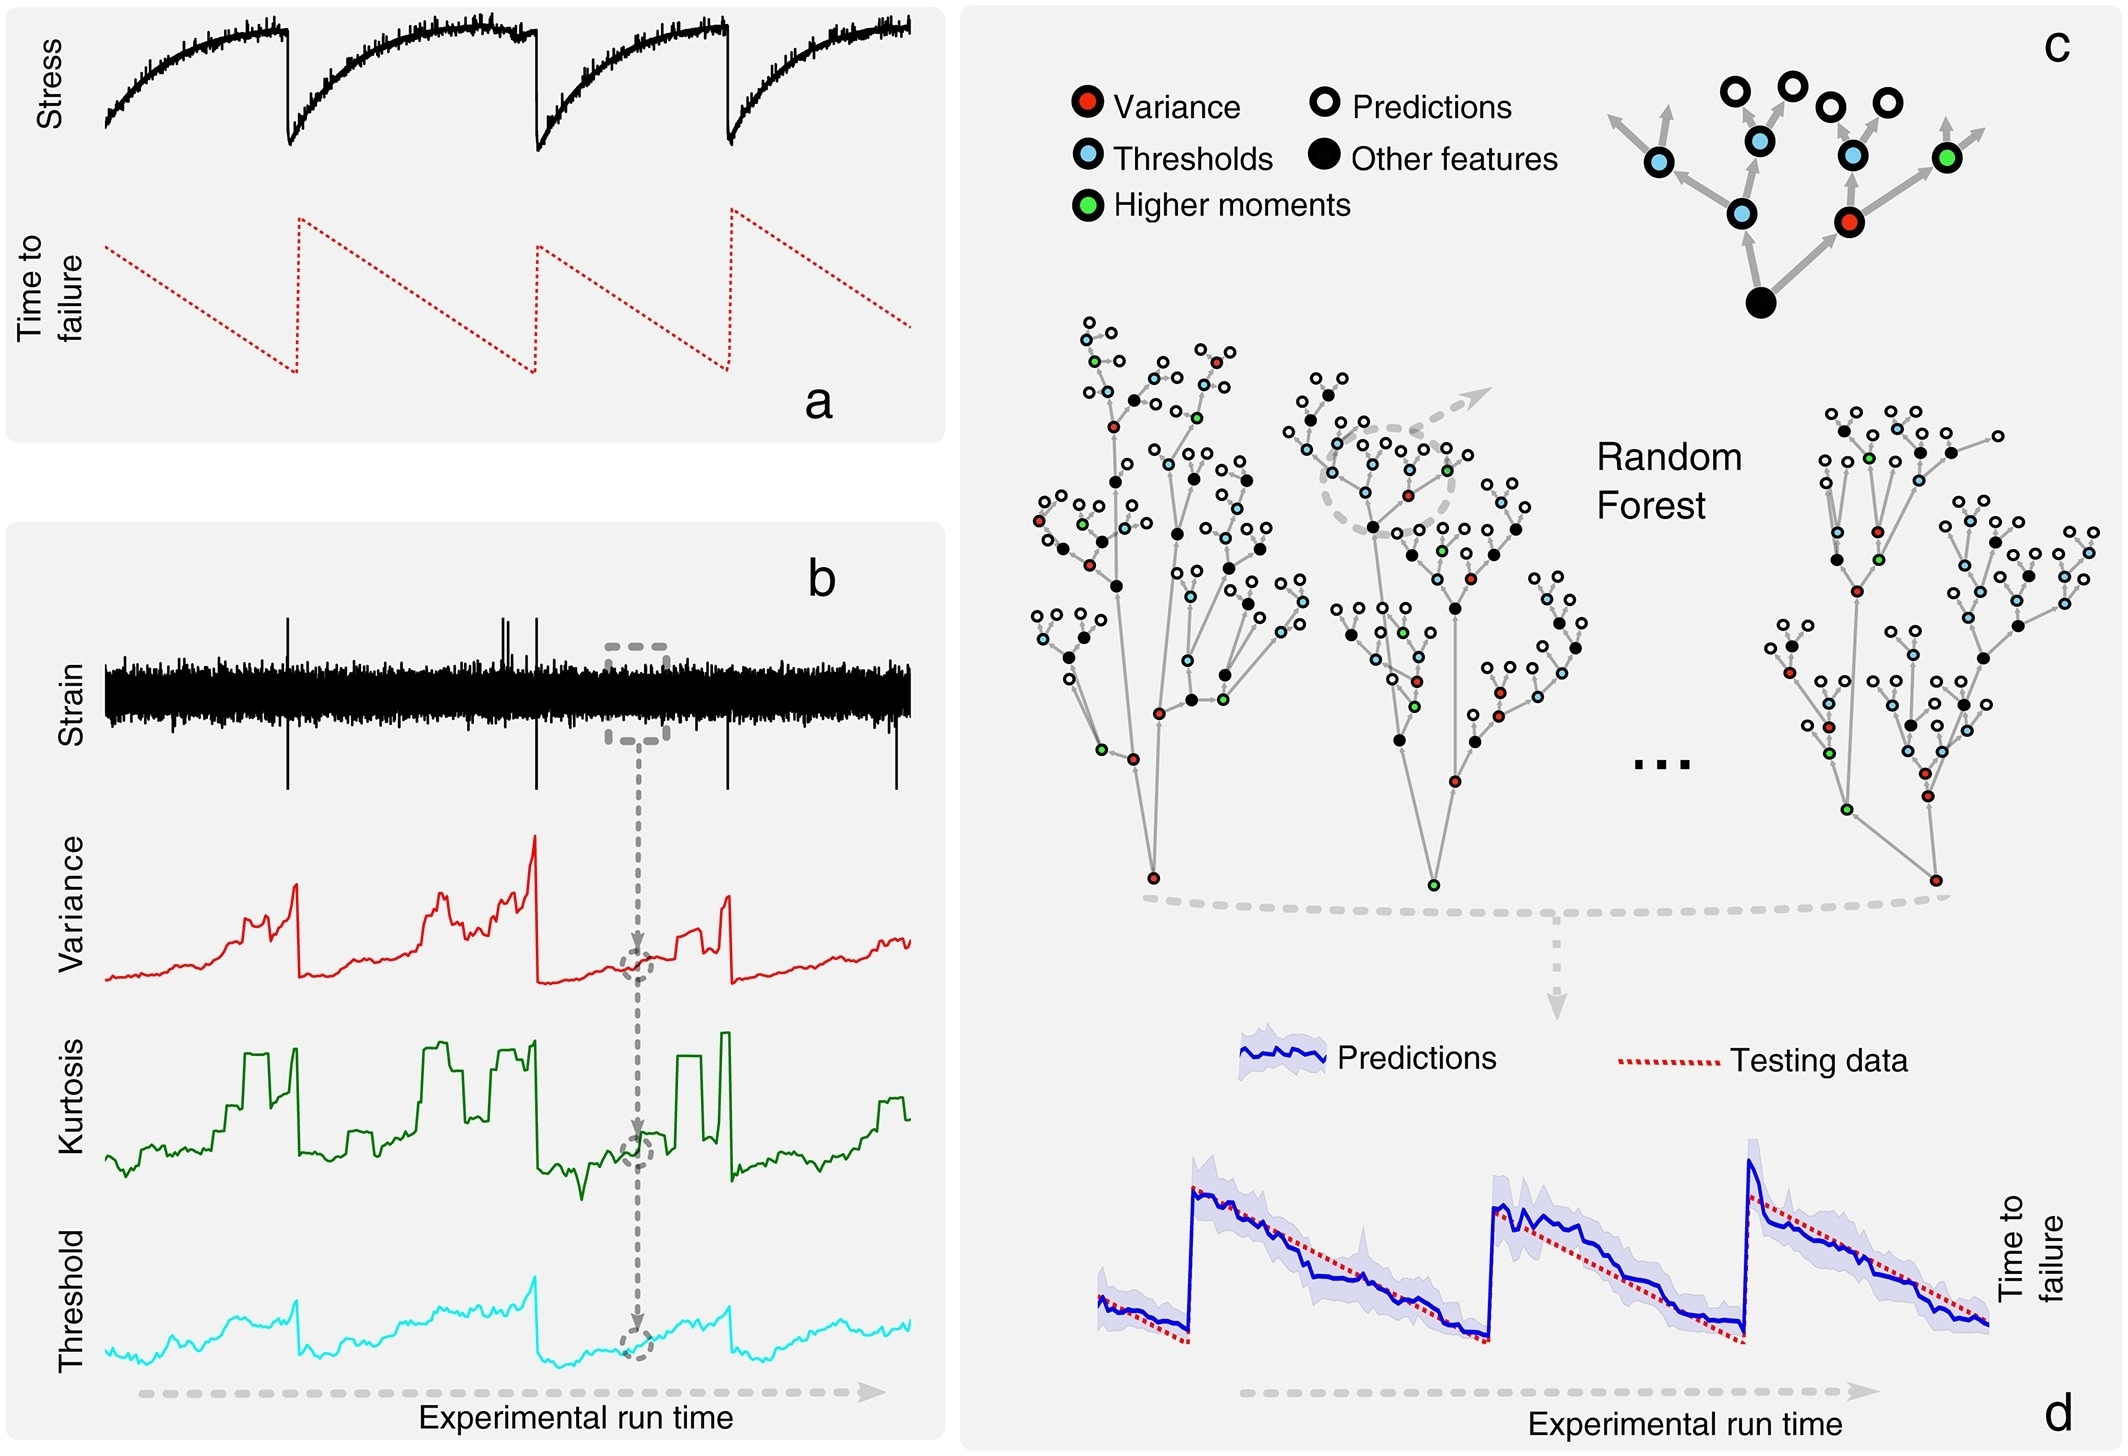
\includegraphics[width=0.7\linewidth]{pictures/grl56367-fig-0001-m.jpg}
	\caption{Random Forest (RF) approach for predicting time remaining before failure.}
	\label{fig:RF1}
\end{figure}

From each time window, a set of approximately 100 statistical features are computed, then selected recursively by usefulness, and lastly used to actually predict the time before the next earthquake. The results achieved through this study are quite accurate, even if it needs to be noted that a laboratory earthquake does not capture the physics of a complex, real-world earthquake.

\begin{figure} [h]
	\centering
	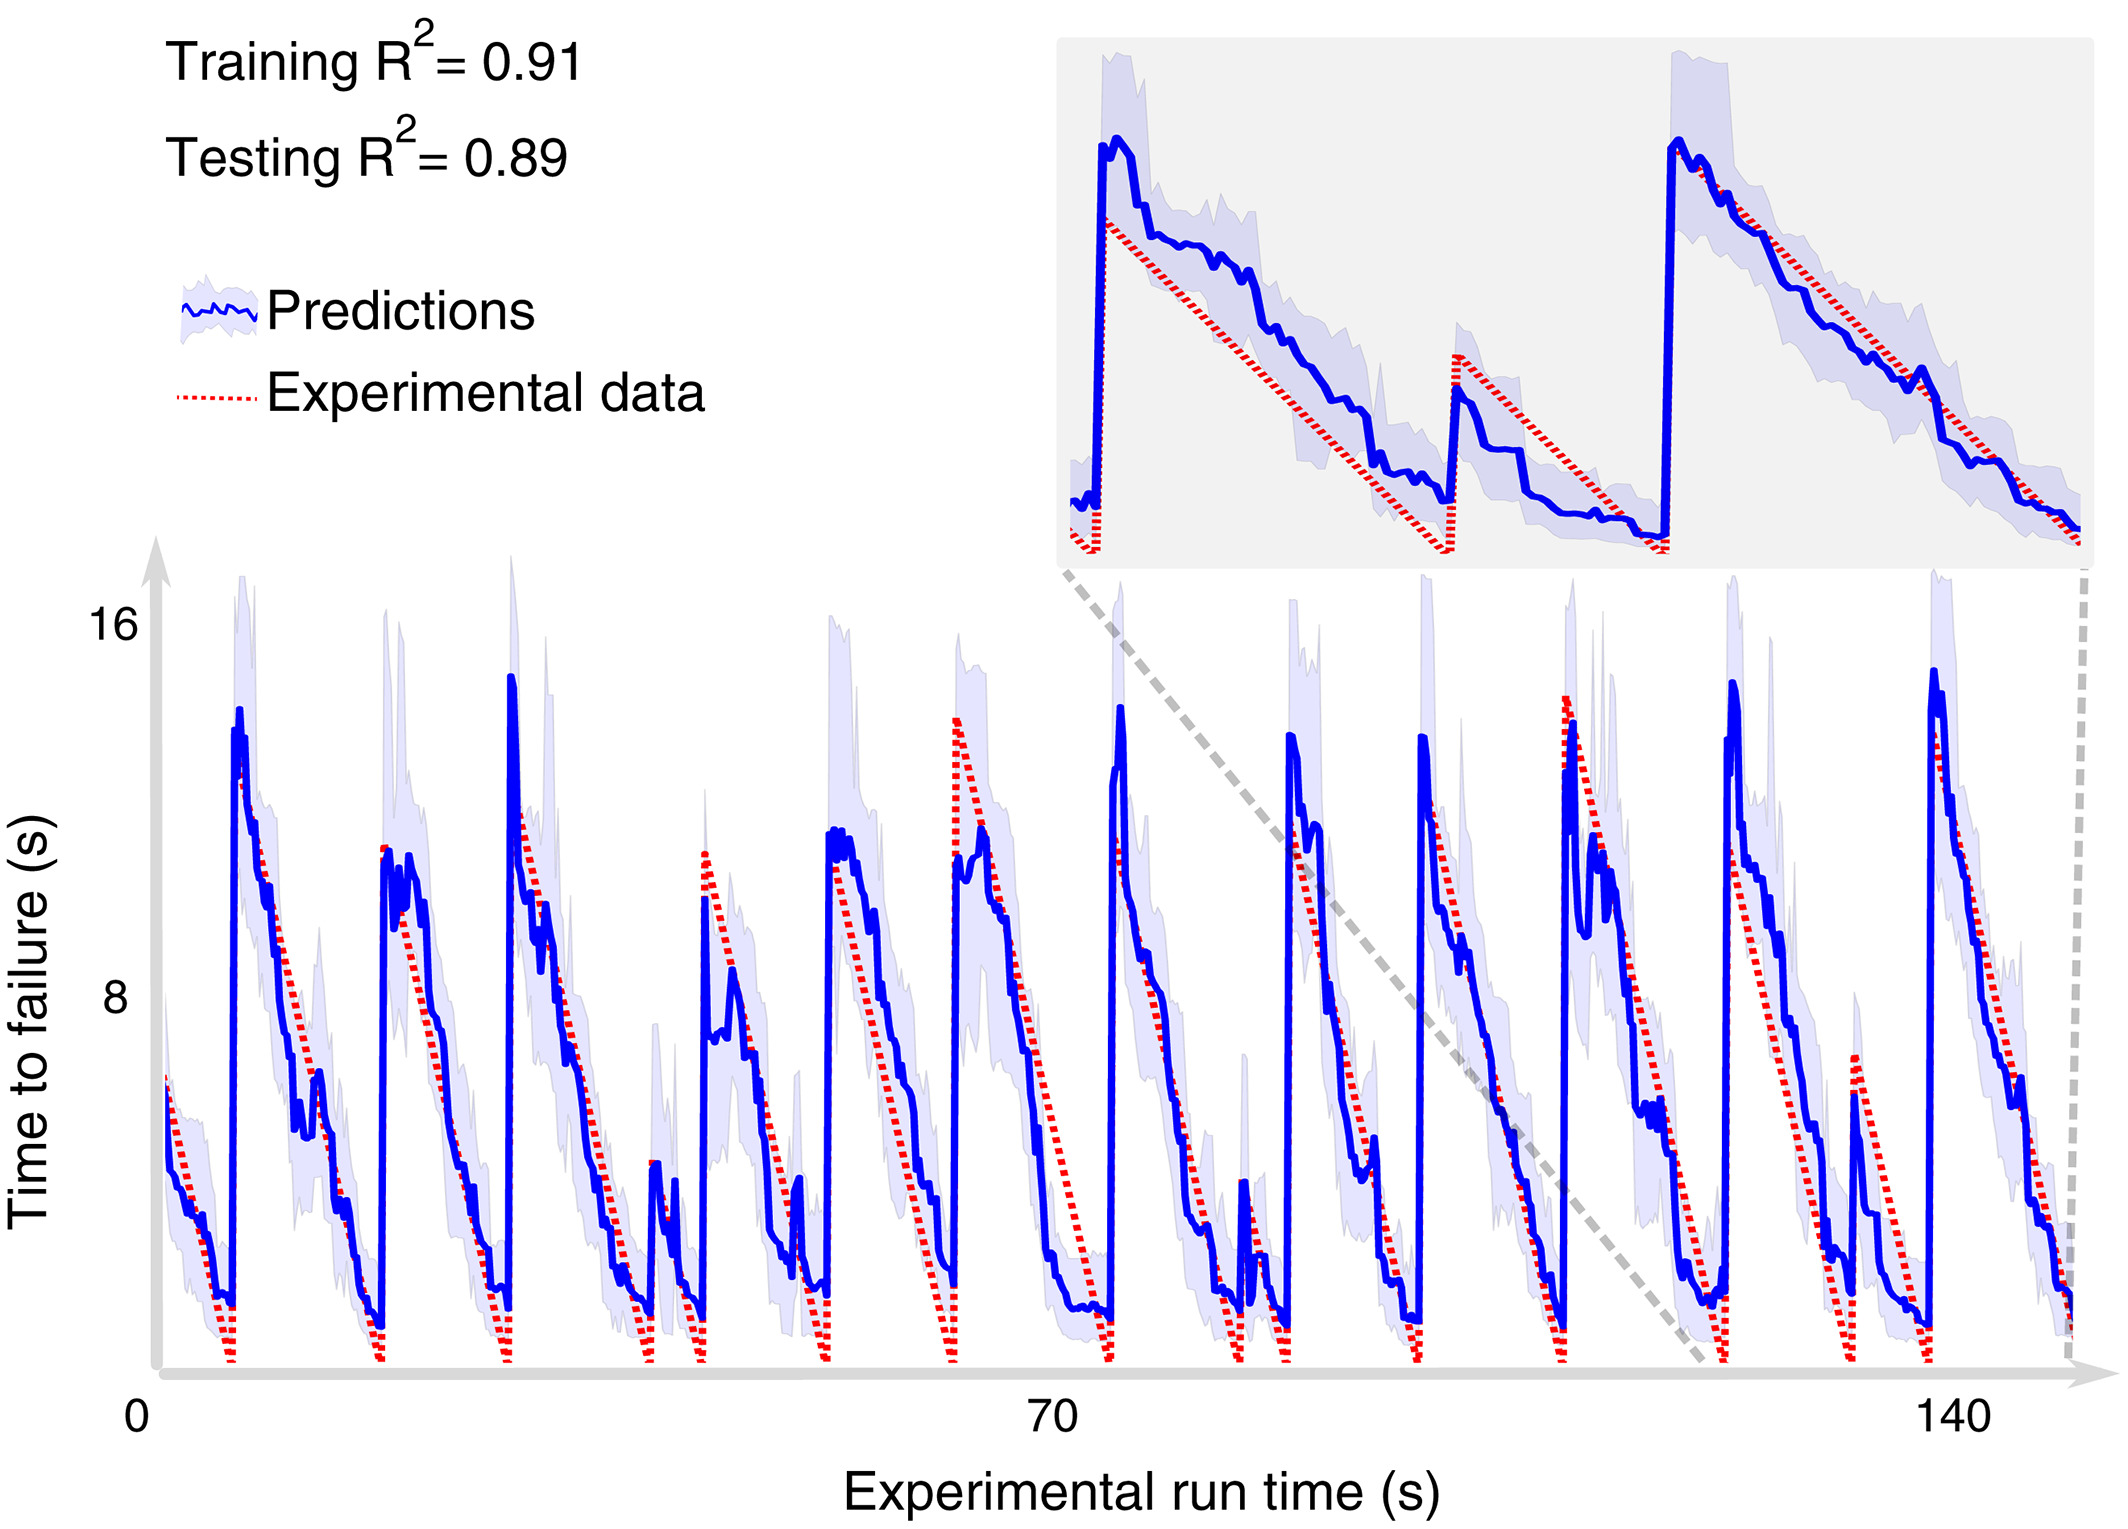
\includegraphics[width=0.7\linewidth]{pictures/grl56367-fig-0002-m.jpg}
	\caption{Time remaining before the next failure predicted by the Random Forest.}
	\label{fig:RF2}
\end{figure}

\section{Understanding the data}
With reference to the above mentioned studies, the dataset provided for the challenge contains more a-periodic occurrences of earthquake hazards, thus resembling more a real-world scenario. The data comes from a well-known experimental set-up used to study earthquake physics \cite{challenge}.

In particular, the dataset is made of two subsets:
\begin{itemize}
	\item \texttt{train.csv} - A single, continuous training segment of experimental data (with 629.145.480 entries);
	\item \texttt{test} - A folder containing many small segments (\texttt{.csv}) of test data (2.624 segments of 150.000 entries each).
\end{itemize}

\noindent Each entry of the training set has two fields:
\begin{itemize}
	\item \texttt{acoustic\textunderscore data} - the seismic signal [\texttt{int16}];
	\item \texttt{time\textunderscore to\textunderscore failure} - the time (in seconds) until the next laboratory earthquake [\texttt{float64}].
\end{itemize}

On the other hand, each segment from the test set folder is named after its \texttt{seg\textunderscore id} and only has one field, the \texttt{acoustic\textunderscore data}.
While the training set is a single, continuous, big segment of experimental data, the test set is continuous within a single segment, but the set of files cannot be considered continuous; thus, the predictions can't be assumed to follow the same pattern of the training file.

The goal of the competition is to predict a single \texttt{time\textunderscore to\textunderscore failure} for each segment, corresponding to the time between the last row of the segment and the next laboratory earthquake. The results must be submitted on the Kaggle platform as a \texttt{.csv} file containing the predictions for each test segment, and the score is then obtained through the application of the \textit{Mean Absolute Error} between the real time values and the predictions.

\bigbreak

A first approach to better understand what the data represents is to plot it (or a part of it, given the prohibitive size of the training set). In picture \ref{fig:plot1} we can see 1\% of the training data (obtained simply by sampling every 100 entries) \cite{kernelpreda}.

\begin{figure} [h]
	\centering
	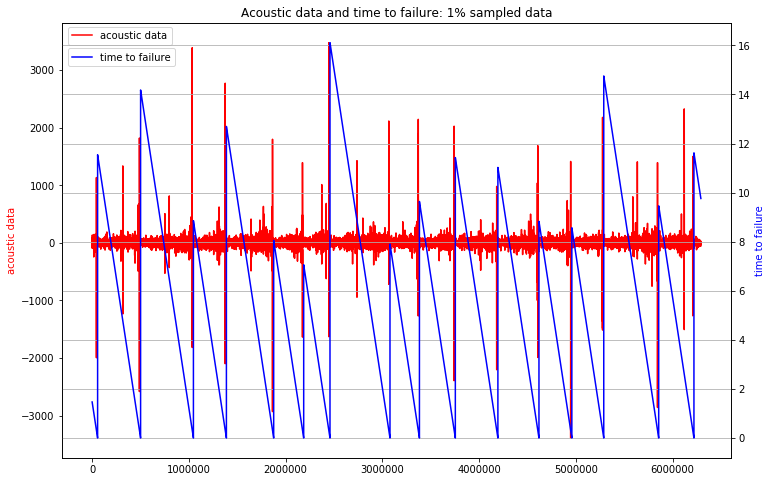
\includegraphics[width=0.7\linewidth]{pictures/plot1.png}
	\caption{Plot of 1\% sampling of the training data}
	\label{fig:plot1}
\end{figure}

The following (\ref{fig:plot2}) is instead the representation of the first 1\% entries of the training dataset: even at a first glance we are able to note that the failure ("\textit{labquake}") occurs after some medium oscillations, a very large one and some other minor ones. 

\begin{figure} [h]
	\centering
	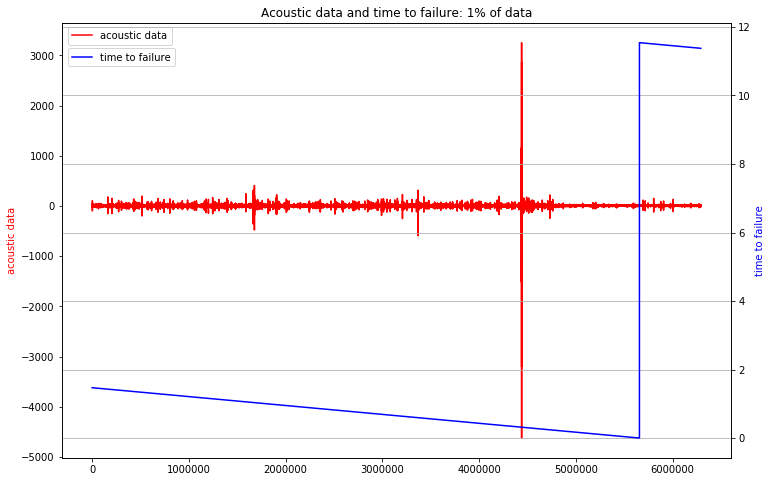
\includegraphics[width=0.7\linewidth]{pictures/plot2.png}
	\caption{Plot of the first 1\% of the training data}
	\label{fig:plot2}
\end{figure}

Before going into further details and taking a first step towards building the model from the training data, it's worth to also take a look at the structure of the test data. In picture \ref{fig:plot3} are represented four of the segments from the test folder \cite{kernelallunia}.

\begin{figure} [h]
	\centering
	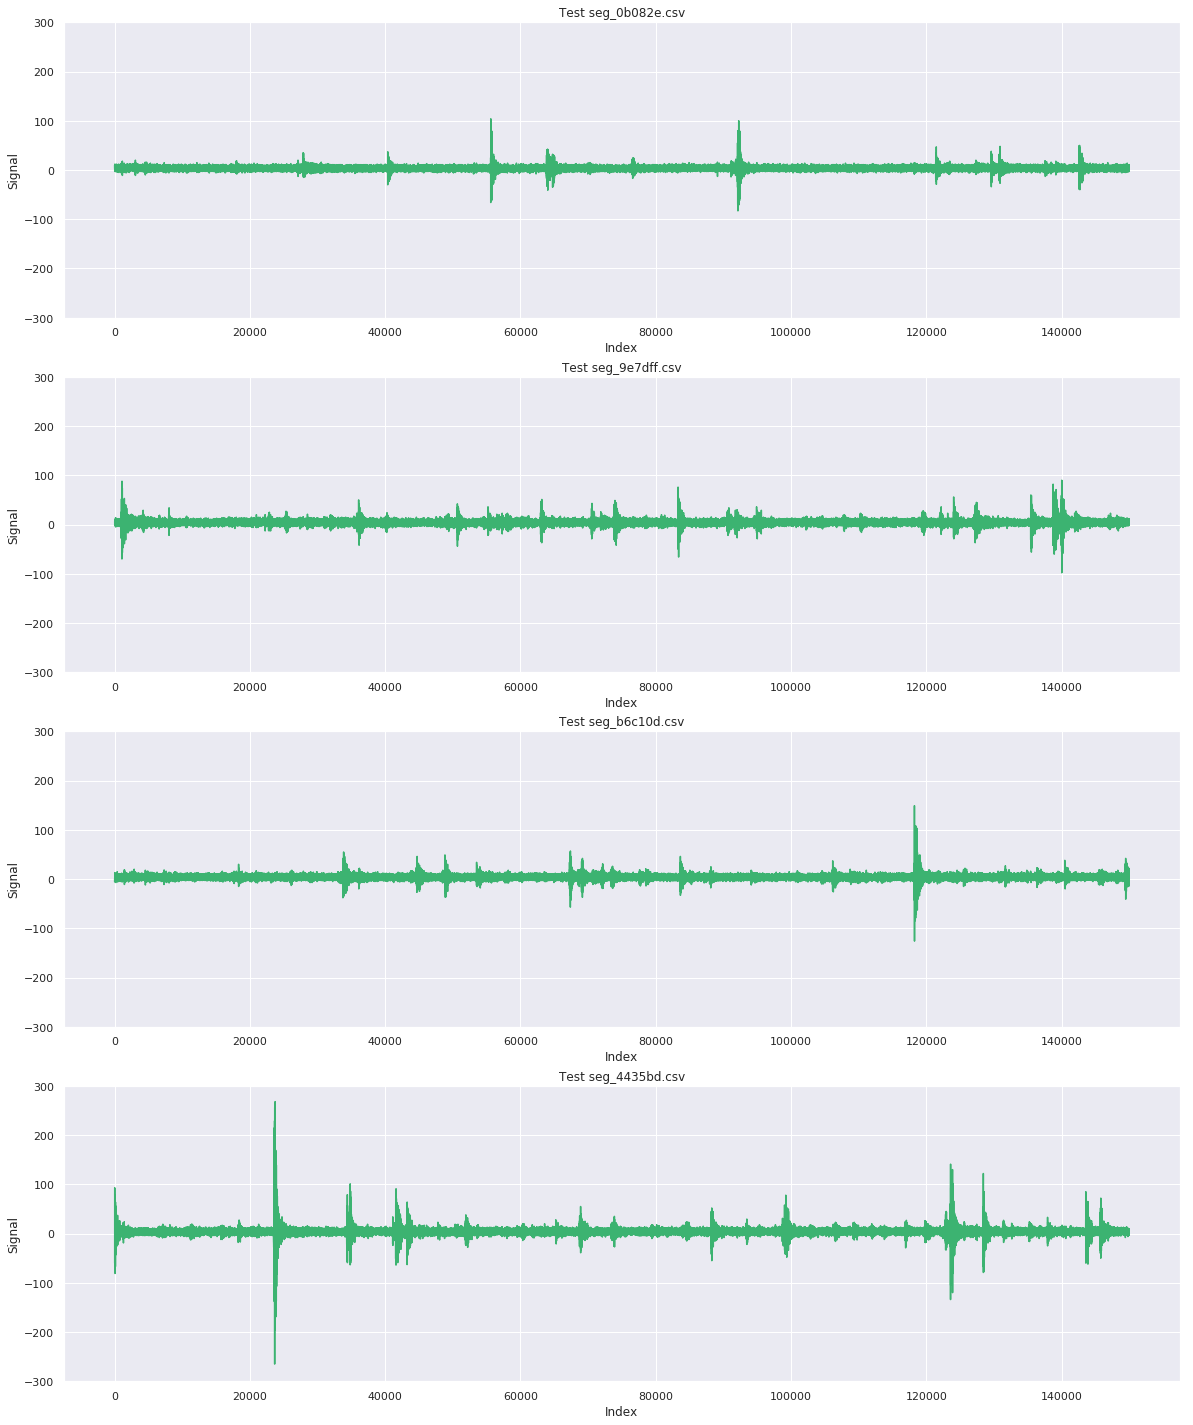
\includegraphics[width=0.7\linewidth]{pictures/plot3.png}
	\caption{Plot of four segments of the test data}
	\label{fig:plot3}
\end{figure}

\bigbreak

Overall, what we can take away from this first dive into the datasets is:
\begin{itemize}
	\item that the task of this Data Mining challenge will be in the regression spectrum, since the output falls in a continuous range rather than a set of discrete classes;
	\item that the dimension of the segments is not that big if compared to the very rare occurrences of laboratory earthquakes;
	\item that these failure events will appear very much like outliers, given the scarcity of representation and the intensity of the acoustic signal when compared to the other values.
\end{itemize}

As others participants to the challenge have noticed, it may be also relevant to note that the test set doesn't contain \textit{any} earthquake: thus, it may be worth considering not including the few failure occurrences that can be found in the training set, to avoid the model trying to match the data to these much higher peaks when fed with the test set.
	\chapter{A first, na{\"i}ve model}
\label{capitolo2}
\thispagestyle{empty}

\noindent A first, very simple approach to building the model for the purpose of this competition is given directly by the promoters of the challenge \cite{kernelinit}.

\bigbreak

Before seeing what the \textit{Python kernel} looks like, it's worth to dig a bit deeper on how the data is prepared for the task. In fact, taking the dataset "as it is", it's easy to notice that it has just one feature (\texttt{acoustic\textunderscore data}) that can be used to compute the regression task of predicting \texttt{time\textunderscore to\textunderscore failure} on the test set.

For this reason, data needs to be prepared: the obvious choice is to divide the training set into chunks of 150.000 rows (the size of each segment of the test set; this is not the only choice available), and for each of them compute some features representing the data; in this first basic solution we will extract the mean, standard deviation, maximum and minimum. The resulting dataset will contain an entry for each portion of the initial dataset, with one column for each computed feature (in this case 4), and another dataset with just the original \texttt{time\textunderscore to\textunderscore failure} associated with the last row of the chunk (similarly to the test segments).

\section{Basic Feature Benchmark}
\begin{lstlisting}
# This Python 3 environment comes with many helpful analytics libraries installed
# It is defined by the kaggle/python docker image: https://github.com/kaggle/docker-python
# For example, here's several helpful packages to load in 

import numpy as np # linear algebra
import pandas as pd # data processing, CSV file I/O (e.g. pd.read_csv)

# Input data files are available in the "../input/" directory.
# For example, running this (by clicking run or pressing Shift+Enter) will list the files in the input directory

import os
print(os.listdir("../input"))

# Any results you write to the current directory are saved as output.
\end{lstlisting}

\begin{lstlisting}[firstnumber=15]
import matplotlib.pyplot as plt
from tqdm import tqdm
from sklearn.preprocessing import StandardScaler
from sklearn.svm import NuSVR
from sklearn.metrics import mean_absolute_error
\end{lstlisting}

\begin{lstlisting}[firstnumber=20]
train = pd.read_csv('../input/train.csv', dtype={'acoustic_data': np.int16, 'time_to_failure': np.float64})
\end{lstlisting}

After these preliminary operations of including the necessary libraries and loading the dataset, we are able to get into the data preparation as previously described. In the following snippet, \texttt{X\_train} is the dataset containing the segments' 4 computed features, while \texttt{Y\_train} contains the associated \texttt{time\textunderscore to\textunderscore failure}.

\begin{lstlisting}[firstnumber=21]
# Create a training file with simple derived features

rows = 150_000
segments = int(np.floor(train.shape[0] / rows))

X_train = pd.DataFrame(index=range(segments), dtype=np.float64,
                       columns=['ave', 'std', 'max', 'min'])
y_train = pd.DataFrame(index=range(segments), dtype=np.float64,
                       columns=['time_to_failure'])

for segment in tqdm(range(segments)):
    seg = train.iloc[segment*rows:segment*rows+rows]
    x = seg['acoustic_data'].values
    y = seg['time_to_failure'].values[-1]
    
    y_train.loc[segment, 'time_to_failure'] = y
    
    X_train.loc[segment, 'ave'] = x.mean()
    X_train.loc[segment, 'std'] = x.std()
    X_train.loc[segment, 'max'] = x.max()
    X_train.loc[segment, 'min'] = x.min()
\end{lstlisting}

The kernel's authors' choice for modeling the solution is to use \textit{Support Vector Regression}. The \texttt{scikit-learn} Python library implementation of SVR recommends explicitly that the data is scaled, since Support Vector Machine algorithms are not scale invariant.

\begin{lstlisting}[firstnumber=42]
scaler = StandardScaler()
scaler.fit(X_train)
X_train_scaled = scaler.transform(X_train)
\end{lstlisting}

\begin{lstlisting}[firstnumber=45]
svm = NuSVR()
svm.fit(X_train_scaled, y_train.values.flatten())
y_pred = svm.predict(X_train_scaled)
\end{lstlisting}

The results predicted are then compared with the actual training data, by computing the \textit{Mean Absolute Error}, and finally the test data is prepared and fed to the model and results are printed to the \texttt{submission.csv} file. As expected, this simple model has a score of 2,314 on the training set (the score on the test set can only be computed by the competition's promoters), which denotes a really bad performance.

\begin{lstlisting}[firstnumber=48]
score = mean_absolute_error(y_train.values.flatten(), y_pred)
print(f'Score: {score:0.3f}')
\end{lstlisting}

\begin{lstlisting}[firstnumber=50]
submission = pd.read_csv('../input/sample_submission.csv', index_col='seg_id')
X_test = pd.DataFrame(columns=X_train.columns, dtype=np.float64, index=submission.index)
\end{lstlisting}

\begin{lstlisting}[firstnumber=52]
for seg_id in X_test.index:
    seg = pd.read_csv('../input/test/' + seg_id + '.csv')
    
    x = seg['acoustic_data'].values
    
    X_test.loc[seg_id, 'ave'] = x.mean()
    X_test.loc[seg_id, 'std'] = x.std()
    X_test.loc[seg_id, 'max'] = x.max()
    X_test.loc[seg_id, 'min'] = x.min()
\end{lstlisting}

\begin{lstlisting}[firstnumber=61]
X_test_scaled = scaler.transform(X_test)
submission['time_to_failure'] = svm.predict(X_test_scaled)
submission.to_csv('submission.csv')
\end{lstlisting}

\begin{figure} [h]
	\centering
	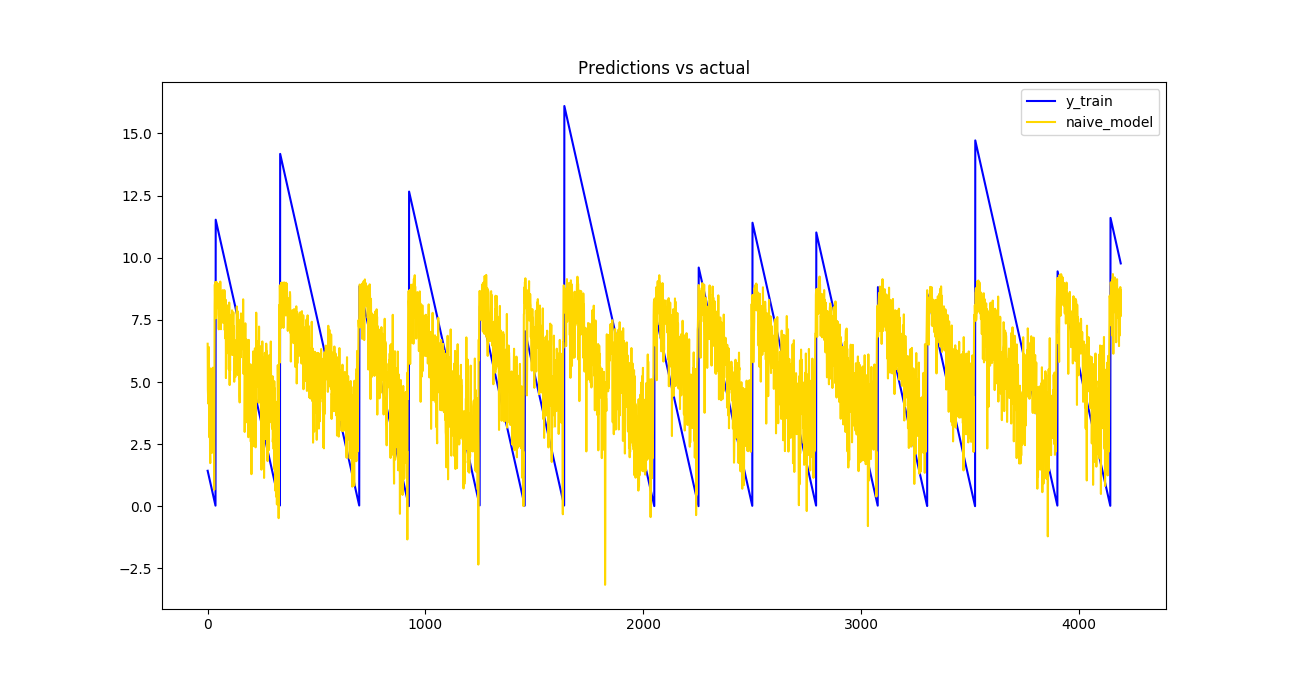
\includegraphics[width=1\linewidth]{pictures/naive.png}
	\caption{Na{\"i}ve model, \texttt{time\textunderscore to\textunderscore failure} predictions vs real values.}
	\label{fig:LR}
\end{figure}
	\chapter{More advanced models comparison}
\label{capitolo3}
\thispagestyle{empty}

\noindent Starting from the basic model presented in the previous section, for the purpose of this project activity we theorized and tested various approaches to solving the problem.

Lasso
Elastic net
Gaussian Probability Regression
Isotonic Regression

\section{First model}


\section{Second model}


\section{Third model}


	\chapter{Infrastructure and tools}
\label{capitolo4}
\thispagestyle{empty}

\noindent Given the nature of the data, even the easiest computation would be really heavy. The sole task of loading \texttt{training.csv} file takes around 3 minutes, and the used RAM amount is about 11 GBs. For this reason, the personal computers physically at our disposal were not enough.

\section[Microsoft Azure VMs]{Microsoft Azure Virtual Machines}
In order to support heavy computations, we signed a subscription on the Microsoft Azure Platform \cite{azure}, that provides students with an initial credit of 100\$, and therefore the possibility to access (some of) their virtual machines.

\begin{figure} [h]
	\centering
	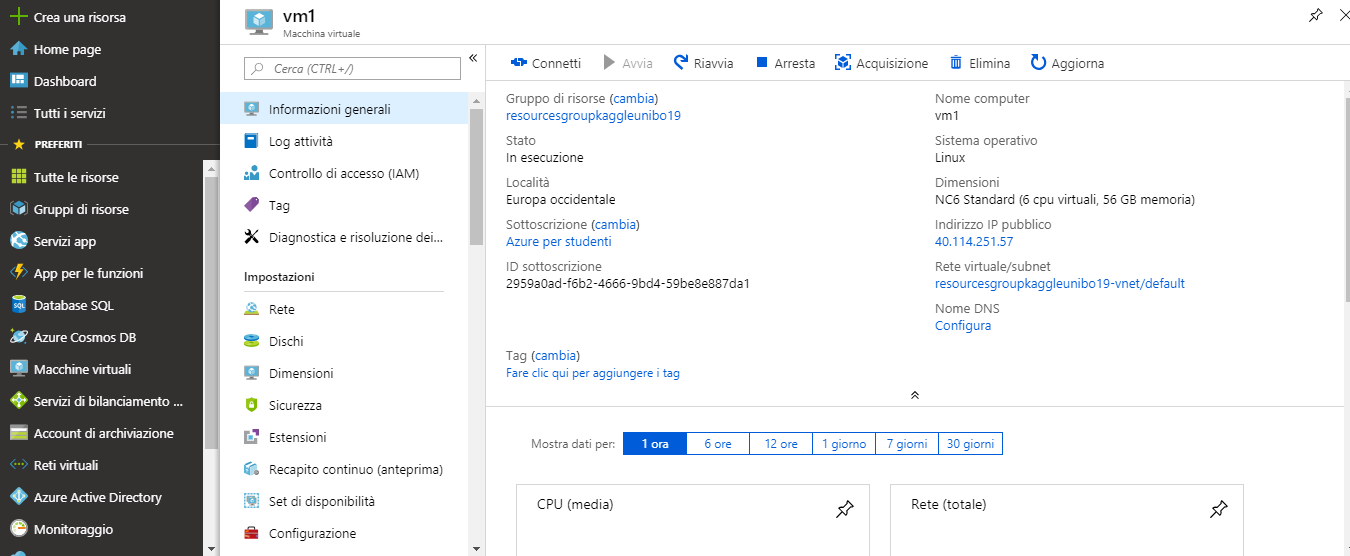
\includegraphics[width=0.9\linewidth]{pictures/azure.png}
	\caption{Azure Platform screenshot.}
	\label{fig:azure}
\end{figure}

According to the limitations given to student accounts, we instantiated the machine with the maximum of cores and GBs of RAM possible, which happened to be the NC6 Standard machine (with 6 virtual CPUs and 56 GBs RAM). Python was already installed on it, and we only had to install the other libraries (like \texttt{scikit-learn}) in order for our scripts to run. Access to the machine was made possible through SSH connection established through the \textit{PuTTY} client installed on our laptops \cite{putty}. Graphic visualization of the plots presented in the report were made available through \textit{Xming} \cite{xming}.

\begin{figure} [h]
	\centering
	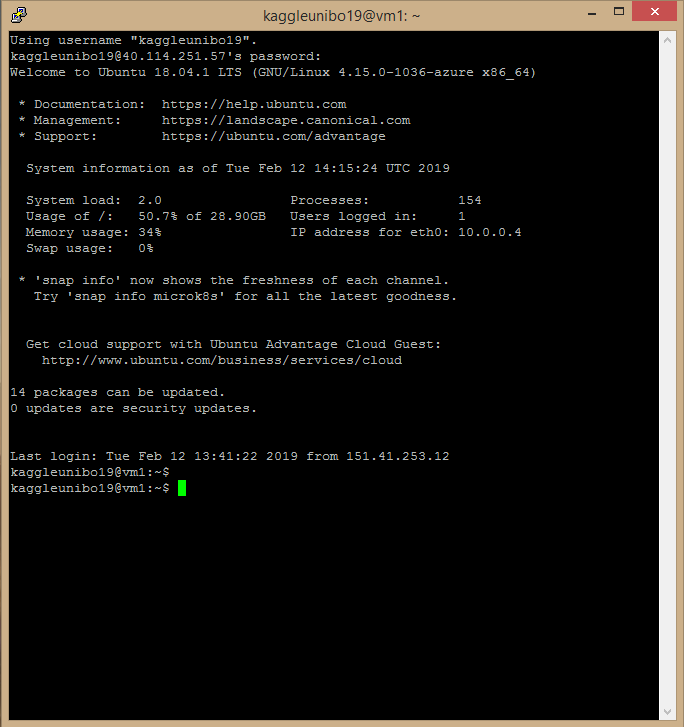
\includegraphics[width=0.7\linewidth]{pictures/cmd.png}
	\caption{Command line with SSH access to the VM.}
	\label{fig:cmd}
\end{figure}

The whole collection of \texttt{.py} scripts explored and the various results obtained have been saved and stored in a repository, available on GitHub \cite{github}.
	\chapter{Conclusions}
\label{conclusioni}
\thispagestyle{empty}

\noindent For this Data Mining project activity we were presented with a simulated seismic data mining problem and the task to predict the time remaining until the next laboratory earthquake; starting from raw data, we pre-processed it by computing aggregated representative data to be fed to a model of our choice. We tested different models from the most used Python library, \texttt{scikit-learn}, starting from the most simple ones up until neural networks, and we encountered various issues that we tried to dig deep into with the intention of understanding them and drawing our conclusions.

Further development of the presented models could be accomplished by tweaking and refining the parameters settings, a task that we did not pursue due to time restrictions, knowledge boundaries, and to our common decision to focus more on exploring different models and collecting the responses.

	\linespread{1}
	\selectfont

	\clearpage{\pagestyle{empty}\cleardoublepage}
	\addcontentsline{toc}{chapter}{Bibliography}
	\bibliographystyle{plainurl}
	\bibliography{bibl_report}

\end{document}
